\section{Non-Gaussian States} 
    A state that does not fulfill the definition \ref{def:Gaussian} is a non-Gaussian state.
    An important and useful for communications class of non-Gaussian states, are the photon 
    added states, examined in this thesis. Lastly will be mentioned another type of non-Gaussian
    state: the photon subtracted state.
    
    \subsection{Photon added states}
        \label{PAS}
        The photon added state $\Operator{\varXi}^{(1)}$, obtained from the quantum state $\Operator{\varXi}$,
        is given by:
        \begin{equation}
            \Operator{\varXi}^{(1)}=\frac{\Operator{A}^\dagger\Operator{\varXi}\Operator{A}}
            {\tr{\Operator{A}^\dagger\Operator{\varXi}\Operator{A}}}.
        \end{equation}
        The name \emph{photon addition} could lead to believe that the mean photon number of the 
        photon added state is icreased by one compared to the previous non photon added state.
        However, that is incorrect.
        In general, its mean number of photons could be the same, more or less than the starting state.
        Only if $\Operator{\varXi}=\ket{n}\bra{n}$, i.e $\Operator{\varXi}$ is the density operator corresponding to
        the Fock state $\ket{n}$, the result of the photon addition is a state with one more photon.

        The photon added state $\Operator{\varXi}^{(k)}$ (with $k$ photon addition) is given by
        \begin{equation}
            \Operator{\varXi}^{(k)}=\frac{(\Operator{A}^\dagger)^k\Operator{\varXi}\Operator{A}^k}
            {\tr{(\Operator{A}^\dagger)^k\Operator{\varXi}\Operator{A}^k}}.
        \end{equation}
        The Fock representation of a photon added state, can be obteined as:
        \begin{equation}
            \Operator{\varXi}^{(k)}=\frac{\tilde{\Operator{\varXi}}^{(k)}}{\tr{\tilde{\Operator{\varXi}}^{(k)}}}
            \label{eq:FR_photonAdded}
        \end{equation}
        and
        \begin{equation*}
            \bra{n}\tilde{\Operator{\varXi}}^{(k)}\ket{m}=
            \begin{cases}
                \sqrt{\frac{n!m!}{(n-k)!(m-k)!}}\bra*{n-k}\pmb{\Xi}\ket*{m-k}\mbox{\ if\ }n,m \geq k\\
                0\mbox{\ otherwise}.
            \end{cases}
        \end{equation*}
        The Wigner W-function of a photon added state is not Gaussian (\ref{def:Gaussian}).

        \paragraph{Photon added coherent states}\mbox{}\\
        Let $\Operator{\varXi}$ be a coherent state of amplitude $\mu \in \mathbb{C}$: 
        \begin{equation*}
            \Operator{\varXi}=\ket{\mu}\bra{\mu}
        \end{equation*}
        the photon added state $\ket*{\mu^{(k)}}$ is called photon added coherent state
        (PACS).
        The Wigner W-function of this state is given by \cite{tesiGuerrini}
        \begin{equation}
            W_+^{(k)}(\alpha) = B_+^{(k)}(\alpha) W_c(\alpha)
        \end{equation}
        where $W_c(\alpha)$ is the Wigner function of the coherent state \ref{eq:WignerCoh} and
        \begin{equation}
            B_+^{(k)}(\alpha) = (-1)^k \frac{2 L_k \left( \absolutevalue{2\alpha-\mu}^2 \right)}
            {\pi L_k \left(-\absolutevalue{\mu}^2 \right)}.
            \label{eq:B_plus}
        \end{equation}

        \begin{figure}[t]
            \begin{center}
                \begin{subfigure}{0.49\textwidth}
                    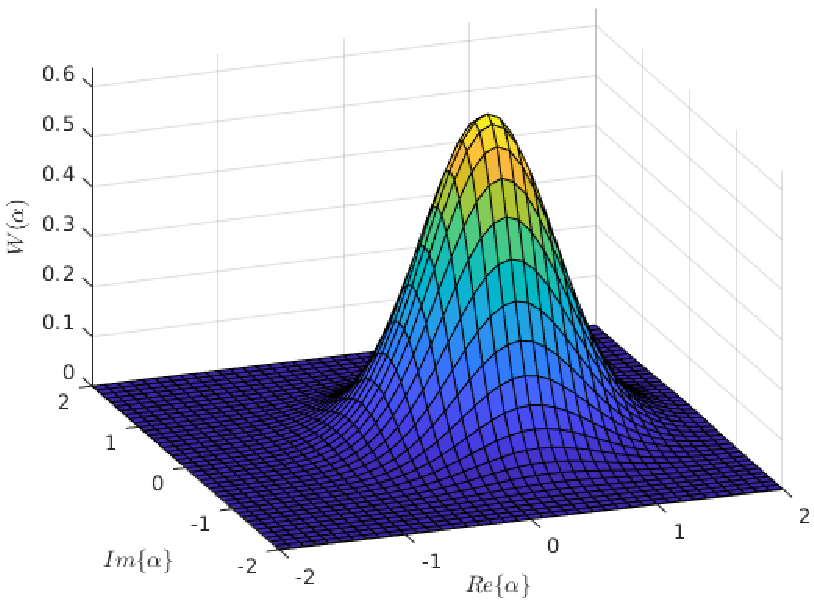
\includegraphics[width=\linewidth]{Pictures/WigCohState.pdf}
                    \caption{Coherent state}
                \end{subfigure}
                \begin{subfigure}{0.49\textwidth}
                    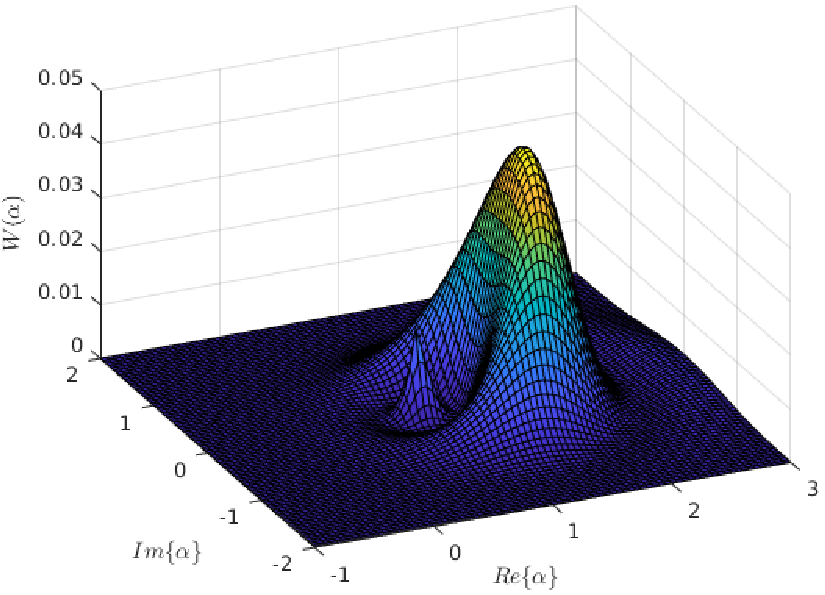
\includegraphics[width=\linewidth]{Pictures/WigPACS.pdf}
                    \caption{PACS}
                \end{subfigure}
                \caption{Comparison between the Wigner W-function of a coherent state and 
                of a PACS with $k=2$.}
                \label{fig:WignerPACS}
            \end{center}
        \end{figure}
        In figure \ref{fig:WignerPACS} are plotted the Wigner W-function of a coherent
        state and of a PACS without noise, for $k=2$. It is evident that the Wigner 
        W-function of the photon added state is not Gaussian.

        If $\Operator{\varXi}$ is a noisy coherent state of amplitude $\mu$ 
        $(\Operator{\varXi}=\Operator{\varXi}_{\mathrm{th}}(\mu))$,
        the photon added state $\Operator{\varXi}_{\mathrm{th}}^{(k)}(\mu)$ is called noisy photon added coherent state
        (noisy PACS).
        The Fock representation can be obtained by \ref{eq:FR_photonAdded} and can be given in closed
        form by \cite{PACSDisc}
        \begin{equation}
            \bra{n}\Operator{\varXi}_{th}^{(k)}(\mu)\ket{m}=
            \begin{cases}
                c_{n,m}^{(k)} \mbox{\ for\ both\ } n,m \geq k\\
                0\mbox{\ otherwise}
            \end{cases}
        \end{equation}
        where
        \begin{equation*}
            c_{n,m}^{(k)}=\frac{(1-v)^{k+1}e^{-(1-v)\absolutevalue{\mu}^2}}{v^k}
            \sqrt{n!}{m!}\binom{m}{k} v^n \left[\left(1-v\right)\mu^*\right]^{m-n}
            \frac{L^{m-n}_{n-k} \left( \frac{-(1-v)\absolutevalue{\mu}^2}{v} \right)}
            {L_k \left( -\absolutevalue{\mu}^2 (1-v) \right)}.
        \end{equation*}
        The Wigner W-function is given by:
        \begin{equation}
            W(\alpha)=\frac{(-1)^k}{(2\bar{n}+1)^k}\frac{L_k \left( 
                \frac{\absolutevalue{2\alpha(\bar{n}+1)-\mu}^2}{(2\bar{n}+1)(\bar{n}+1)} \right)}
                {L_k \left(-\frac{\absolutevalue{\mu}^2}{\bar{n}+1} \right)} W_{th}(\alpha)
        \end{equation}
        where $W_{\mathrm{th}}(\alpha)$ is the Wigner W-function of a noisy coherent state \ref{WignerNCS}.
        
        \paragraph{Photon added squeezed states}\mbox{}\\
        Let $\Operator{\varXi}$ be a squeezed state of amplitude $\mu$ and squeezing parameter $\zeta$,
        with $\mu,\zeta \in \mathbb{C}$:
        \begin{equation*}
            \Operator{\varXi}=\ket*{\mu,\zeta}\bra*{\mu,\zeta}.
        \end{equation*}
        The Wigner W-function of this state is given by
        \begin{equation}
            W_+^{(k)}(\alpha) = B_+^{(k)}(\alpha) W_s(\alpha),
        \end{equation}
        where $W_s(\alpha)$ is the Wigner function of the squeezed state, as given in 
        \ref{eq:WignerSS}, and $B_+^{(k)}(\alpha)$ is 
        given in \ref{eq:B_plus}.
        The Wigner function of the PASS, as that of PACS, is not Gaussian.

        if $\Operator{\varXi}$ is a noisy squeezed state with amplitude $\mu$ and squeezing factor 
        $\zeta$ $(\Operator{\varXi}=\Operator{\varXi}_{\mathrm{th}}(\mu,\zeta))$, the photon added state 
        $\Operator{\varXi}_{\mathrm{th}}^{(k)}(\mu,\zeta)$ is called noisy photon added squeezed state 
        (PASS).

    \subsection{Photon subtracted states}
        Another class of non-Gaussian states are the photon subtracted states. Similarly to PASs, a PSS 
        $\ket*{\psi_-}$ can be obtained from a generic quantum state $\ket*{\psi}$ as
        \begin{equation}
            \ket*{\psi_-} = \frac{\Operator{A}^k \ket{\psi}}{\sqrt{\bra{\psi}(\Operator{A}^\dagger)^k\ket{\psi}}}.
        \end{equation}
        As in PASs the name \emph{photon subtraction} can not be interpreted in deterministic sense.
        It is also important to notice that if $\ket{\psi}=\ket{\mu}$, i.e. the state $\ket{\psi}$ is 
        a coherent state, the photon subtraction has not effect, that is:
        \begin{equation*}
            \ket*{\psi_-}=\ket{\mu}.
        \end{equation*}